% vim:encoding=utf8 ft=tex sts=2 sw=2 et:

\documentclass{classrep}
\usepackage[utf8]{inputenc}
\usepackage[a4paper, margin=1in]{geometry}
\usepackage{graphicx}

\studycycle{Informatyka, studia zaoczne, inż I st.}
\coursesemester{IV}

%\coursename{Angelologia teoretyczna i stosowana}
\coursename{Inteligentna Analiza Danych}
\courseyear{2016/2017}

\courseteacher{dr. Stasiak}
\coursegroup{sobota, 14:45}

\author{
  \studentinfo{Natalia Mateuszuk}{203940} \and
  \studentinfo{Adrian Grzelak}{200242}
}

\title{Zadanie 3: Algorytmy grupowania obiektów}

\begin{document}

\maketitle

\section{Wprowadzenie}
Celem zadania było zaimplementowanie algorytmów grupowania obiektów. Wybrane zostały algorytmy k-Średnich oraz algorytm Gazu Neuronowego. Dla pewnego 2-wymiarowego zbioru danych zostały przeprowadzone 3 eksperymenty z wykorzystaniem powyższych algorytmów 

\section{Eksperyment 1}
W pierwszym eksperymencie wykorzystamy algorytm k-Średnich. Spróbujemy dobrać adaptacyjnie na podstawie otrzymanego błędu kwantyzacji, ilość środków skupień dla algorytmu z zakresu 2..10. Program po przeprowadzeniu tak zdefiniowanego eksperymentu zwraca wynik :
\scriptsize
\begin{verbatim}
=====================================================================================================
EKSPERYMENT 1
=====================================================================================================
Srodki skupien: 2	Bledy kwantyzacji: 4.780 4.780 4.780 4.780 4.780 	Srednia z prob: 4.780
Srodki skupien: 3	Bledy kwantyzacji: 3.995 3.995 3.995 3.995 3.995 	Srednia z prob: 3.995
Srodki skupien: 4	Bledy kwantyzacji: 3.486 3.486 3.486 3.486 3.486 	Srednia z prob: 3.486
Srodki skupien: 5	Bledy kwantyzacji: 3.131 3.132 3.132 3.132 3.132 	Srednia z prob: 3.131
Srodki skupien: 6	Bledy kwantyzacji: 2.913 2.914 2.908 2.925 2.921 	Srednia z prob: 2.916
Srodki skupien: 7	Bledy kwantyzacji: 2.684 2.682 2.710 2.709 2.679 	Srednia z prob: 2.693
Srodki skupien: 8	Bledy kwantyzacji: 2.468 2.467 2.468 2.467 2.467 	Srednia z prob: 2.467
Srodki skupien: 9	Bledy kwantyzacji: 2.326 2.326 2.344 2.335 2.336 	Srednia z prob: 2.334
Srodki skupien: 10	Bledy kwantyzacji: 2.196 2.194 2.237 2.206 2.214 	Srednia z prob: 2.209
=====================================================================================================
Najmniejszy blad kwantyzacji uzyskalismy dla k = 10. Wynosi on srednio  2.209
Rysunek został uzyskany po 133 iteracjach
=====================================================================================================
\end{verbatim}
\normalsize

\begin{center}
	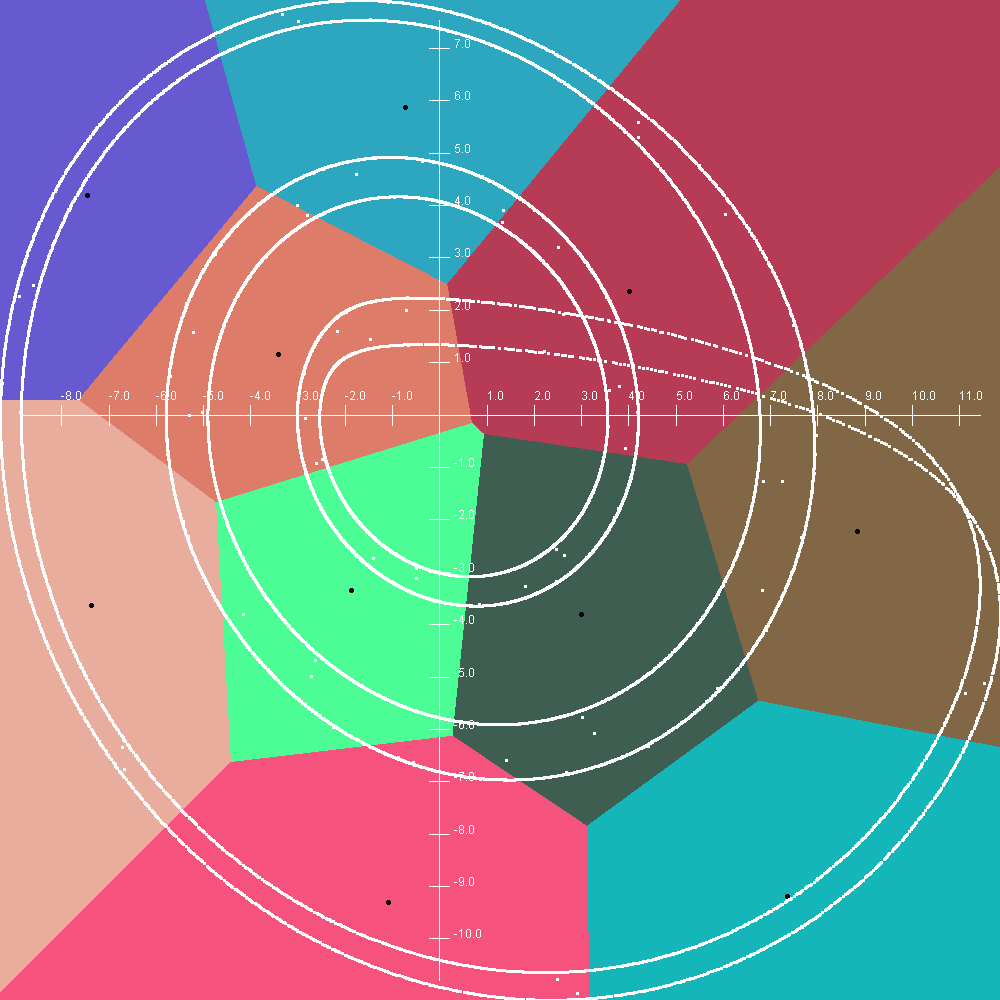
\includegraphics[height=11cm]{kSrednich.png}
	
	
	\textbf{Rysunek 1.} Voronoi Diagram otrzymany dla k-średnich
\end{center}


\section{Eksperyment 2}
W drugim eksperymencie wykorzystamy algorytm Gazu Neuronowego. Podzielimy obszar na tyle samo części co w przypadku najlepszym (10 grup) z poprzedniego eksperymentu. Tak zdefiniowany eksperyment zwraca nam wynik:

\scriptsize
\begin{verbatim}
=====================================================================================================
EKSPERYMENT 2
=====================================================================================================
Blad kwantyzacji dla algorytmu gazu neuronowego wynosi: 2.240
=====================================================================================================
\end{verbatim}
\normalsize

\begin{center}
	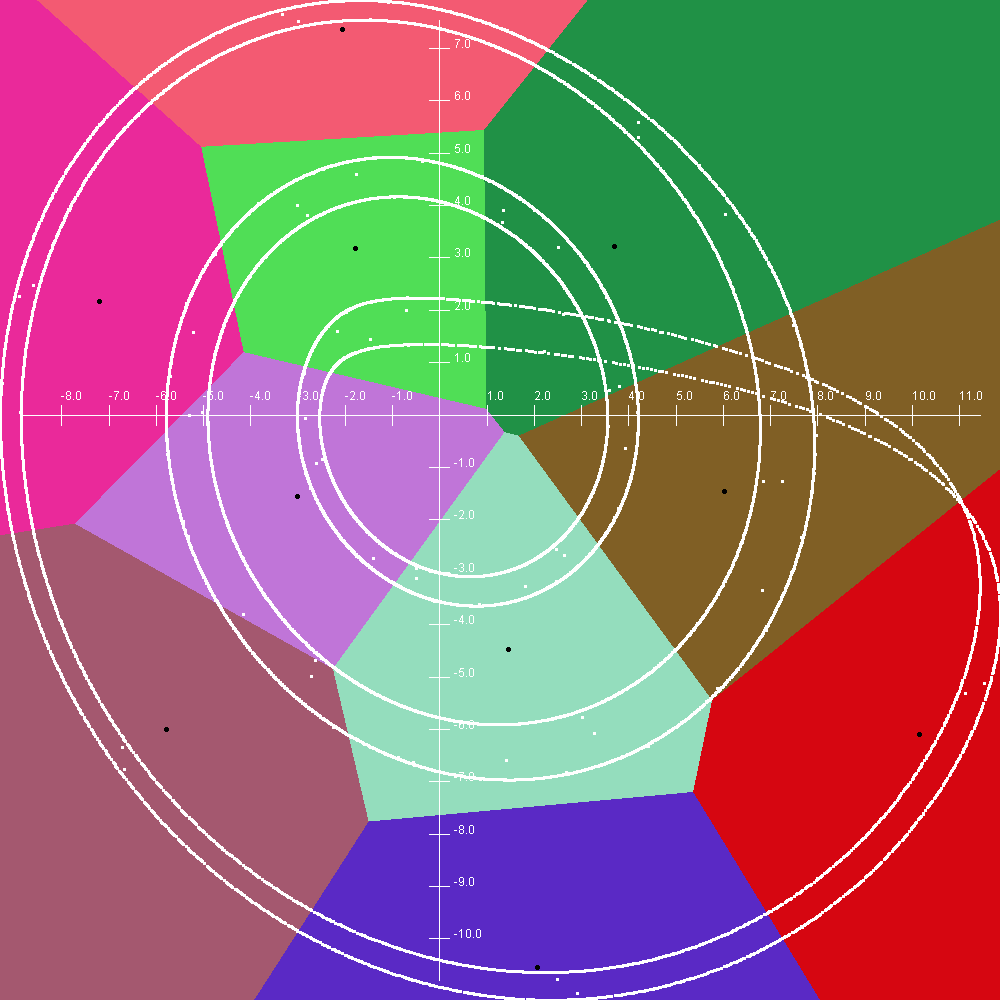
\includegraphics[height=11cm]{gazNeuronowy.png}
	
	
	\textbf{Rysunek 2.} Voronoi Diagram otrzymany dla algorytmu Gazu Neuronowego
\end{center}

\section{Eksperyment 3}

W trzecim eksperymencie dokonamy najpierw podziału obszaru (przy pomocy algorytmu Gazu Neuronowego) na znacznie więcej grup niż w przypadku eksperymentu 1 i 2 (na 100 grup) (Krok 1). Następnie tak otrzymany zbiór wektorów przy pomocy algorytmu k-Średnich znowu pogrupujemy w 10 grup (Krok 2). I ostatecznie porównamy grupowanie z początkowym zbiorem (Krok3). Tak zdefiniowany eksperyment zwraca wynik:

\scriptsize
\begin{verbatim}
=====================================================================================================
EKSPERYMENT 3
=====================================================================================================
W pierwszym kroku podzielilismy na 100 obszarow. Blad kwantyzacji wynosi 0.459
W drugim kroku podzielilismy otrzymany zbior na 10 obszarow. Blad kwantyzacji dla tego kroku wynosi 2.277
Blad kwantyzacji dla calego algorytmu 'mieszanego ;)' wynosi: 2.301
=====================================================================================================
\end{verbatim}
\normalsize

\begin{center}
	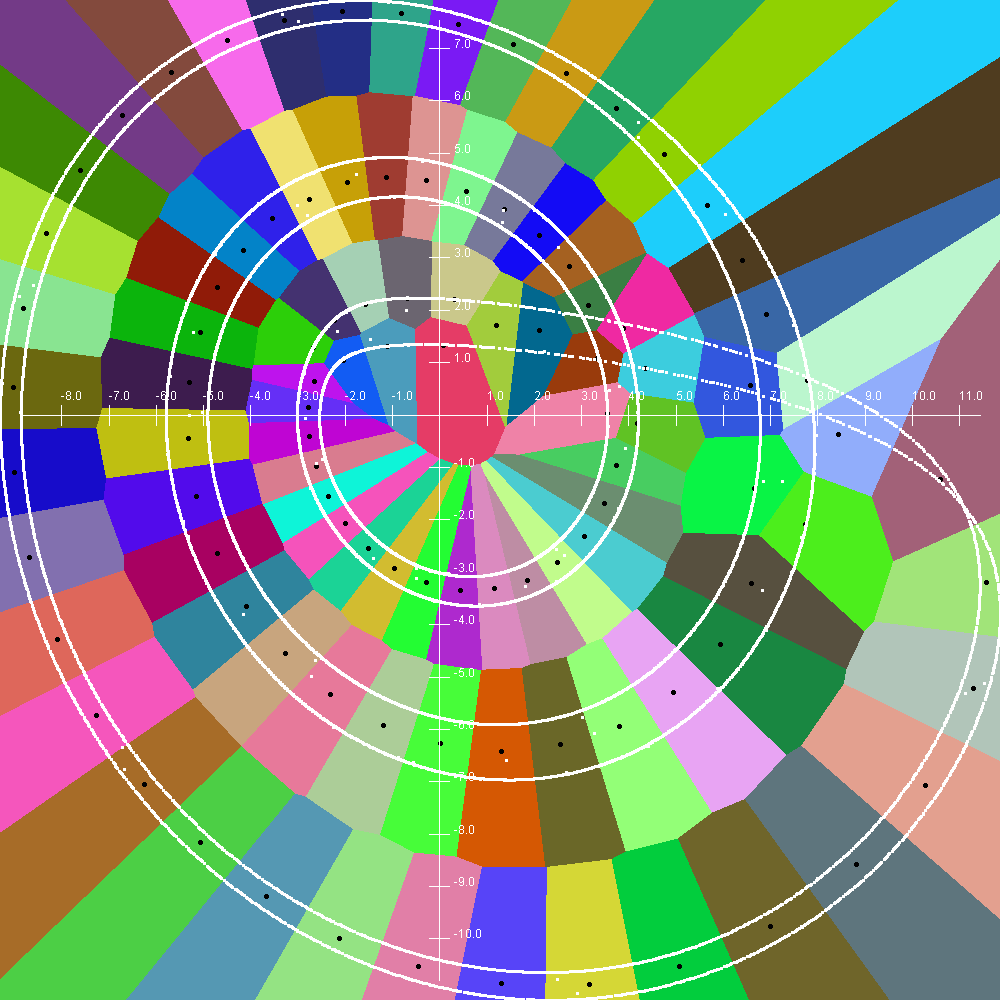
\includegraphics[height=11cm]{mieszany1.png}
	
	
	\textbf{Rysunek 3.} Voronoi Diagram otrzymany po pierwszym kroku
\end{center}

\begin{center}
	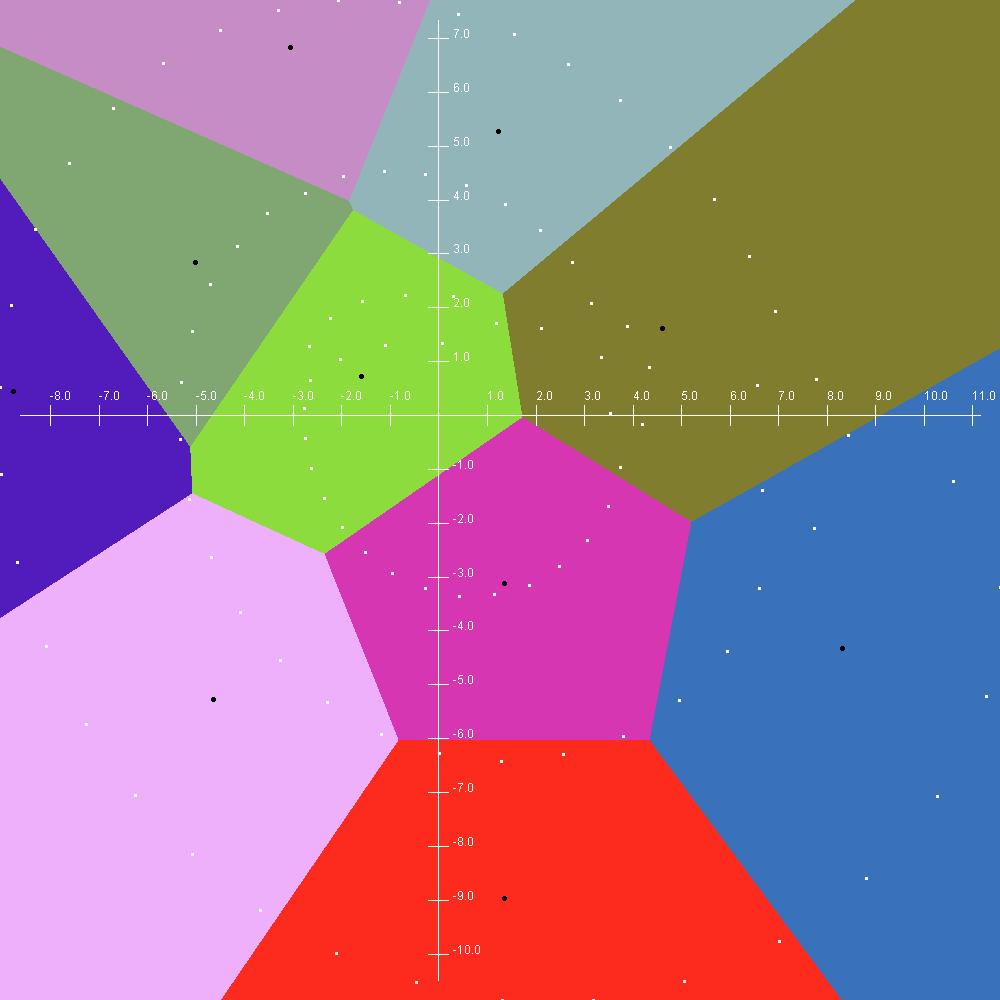
\includegraphics[height=11cm]{mieszany2.png}
	
	
	\textbf{Rysunek 4.} Voronoi Diagram otrzymany po drugim kroku
\end{center}

\begin{center}
	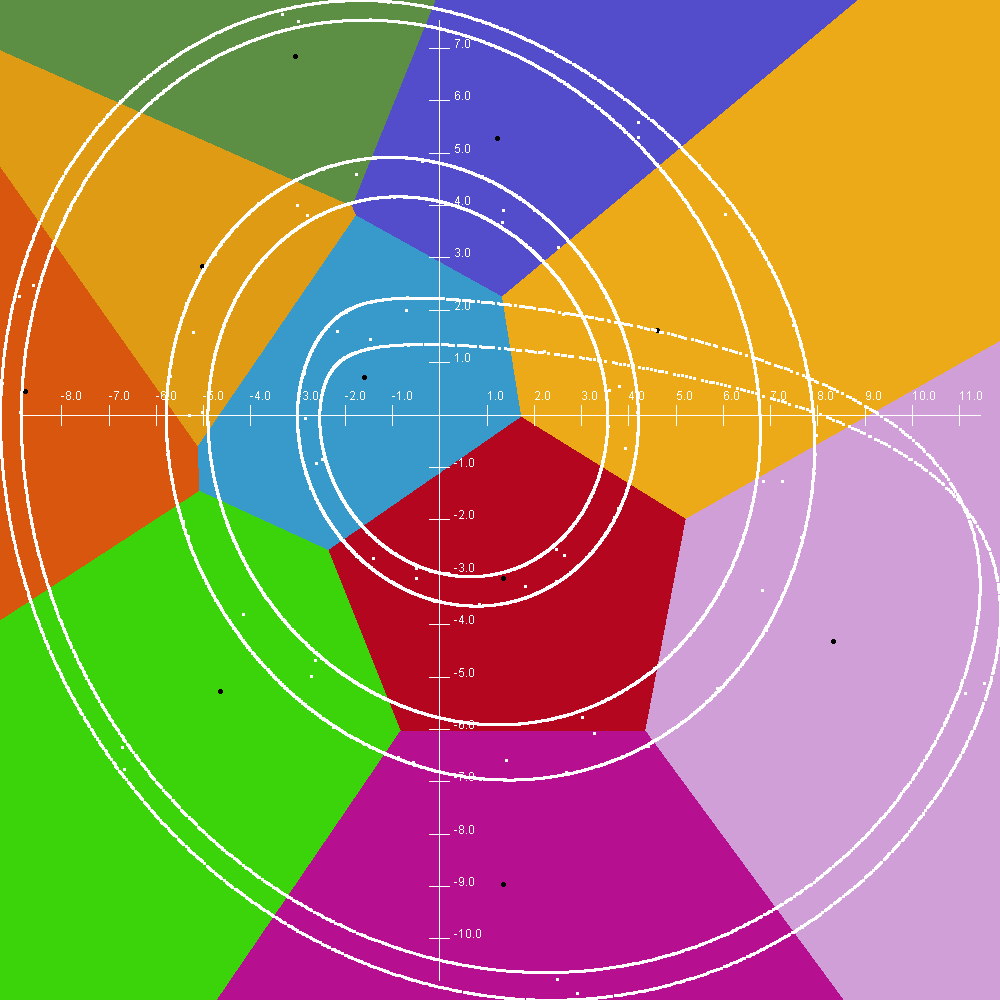
\includegraphics[height=11cm]{mieszany3.png}
	
	
	\textbf{Rysunek 5.} Voronoi Diagram otrzymany po trzecim kroku
\end{center}

\section{Wnioski}
W pierwszym eksperymecie otrzymaliśmy najmniejszy błąd kwantyzacji. W dodatku algorytm k-Średnich ma niską złożoność a co za tym idzie wynik otrzymaliśmy znacznie szybciej niż przy pomocy algorytmu Gazu Neuronowego. Jednakże przy wyborze różnych punktów startowych, nasze diagramy różnią się od siebie, algorytm ten nie daje jednoznacznych wyników. Algorytm Gazu Neuronowego natomiast daje bardziej przybliżone do siebie wyniki, błąd kwantyzacji jest nieco większy, ale odchylenie standardowe wyników jest mniejsze. Możemy wnioskować że algorytm ten daje nam bardziej wiarygodne wyniki. Algorytm mieszany nie daje najlepszych wyników, wynika to z faktu że zbiór otrzymany po pierwszym kroku nie określa tak dobrze zbioru testowanego.



\end{document}
